\section{Experimental results}
Many real world datasets contain missing values, often encoded as blanks, NaNs or other placeholders. Missing data imputation (MDI) is since long a popular problem in statistic and machine learning~\cite{little1986statistical, nelwamondo2007missing}, and recently GNNs have proved to be a powerful predictive tool~\cite{spinelli2020neural}. With a view that our method incorporates additional higher-dimensional structure in the data, we evaluate the performance of the SNNs in imputing missing data on simplicial complexes.

\subsection{Dataset description}
The datasets we analyze has been scraped from the Semantic Scholar Open Research Corpus~\cite{ammar18NAACL}. The data contains over 39 million published research papers in Computer Science, Neuroscience, and Biomedical science together with their authors and number of citations. We retained papers with more than $5$ citations and at most $10$ authors. An important step in preprocessing many kinds of input data in TDA is constructing a simplicial complex. Our work focus on \emph{co-authorship complexes} (or \emph{collaboration complexes})~\cite{patania2017}, simplicial complexes where a paper with $k$ authors is represented by a $(k-1)$-simplex. We constructed different co-authorship complexes by considering sub-samplings from the papers set of the Semantic Scholar dataset. The sub-samplings were obtained by performing random walks (of length $80$) on the nodes of the graph which vertices corresponds to papers and edges connect papers sharing at least one author. The co-authorship complexes obtained from each sub-sampling have corresponding $k$-cochains given by the number of shared citations of the $k$-collaborations (see Figure~\ref{fig:data2complex}).

\subsection{Method}
We evaluate the performance of the SNNs on the task of imputing missing data on the $k$-cochains ($k=0,1,2$) of the extracted co-authorship complexes. As in a typical pipeline for this task~\cite{nelwamondo2007missing}, in our approach missing data is artificially introduced by replacing a portions of the values with a constant. Specifically, given a fixed co-authorship complex missing data is introduced at random on the $k$-cochains at $4$ levels: $10\%,  20\%,  30\%$, and $50\% $. The training input is then given by the $k$-cochains where the random missing data is substituted by the median of the known data. We trained an SNN composed by $3$-layers with $30$ convolutional filters of degree $5$. We used the $L_1$ norm as reconstruction loss over the known elements an the Adam optimizer with learning rate of $1\times 10^{-3}$. The SNN was trained for $1000$ iterations. We then test the performance of the network on its accuracy in imputing missing data. A missing citation is predicted correctly if the imputed value differs of at most $1$ from the actual citation. The accuracy is defined as the percentage of missing values that has been correctly imputed and the absolute error (AE) as the magnitude of the difference between the predicted and actual citation. For the same percentage of missing values we consider different random samples of the damaged portions. Then a statistical evaluation of the performance of the network is given by the mean accuracy (MA), the mean of the accuracy over different samples and the mean absolute error (MAE), the mean of error over different samples.

\subsection{Results}
\gard{Note for me to remember to add a punchline somewhere in this section :-)}

The results in Figure~\ref{fig:accuracy-error} (a-b) show the MA and MAE of the SNN in inputing missing citations on CC1 (Co-authorship Complex 1, for statistics on the complex see Table~\ref{table:Simplices-coauthor}). Observe that the distribution of the prediction error accumulates close to zeros.
\begin{table}[htbp]\label{table:Simplices-coauthor}
  \centering
  \scriptsize{
  \begin{tabular}{llllllllllll}
    \cmidrule(r){1-12}
    Dimension:   & 0     & 1  & 2     & 3 & 4     & 5 & 6    & 7 & 8   & 9 & 10\\
    \midrule
    CC1 & 352  & 1474  & 3285  & 5019  & 5559  & 4547  & 2732  & 1175  & 343 & 61 & 5\\
    CC2 & 1126 & 5059 & 11840 & 18822 & 21472 & 17896  & 10847 & 4673 & 1357 & 238 & 19\\ 
    \bottomrule
  \end{tabular}}
  \vspace{2pt}
  \caption{%
  Number of simplices in co-authorship complexes from the Semantic Scholar dataset.
  }
\end{table}
%\begin{figure}[htbp]
%  \centering
%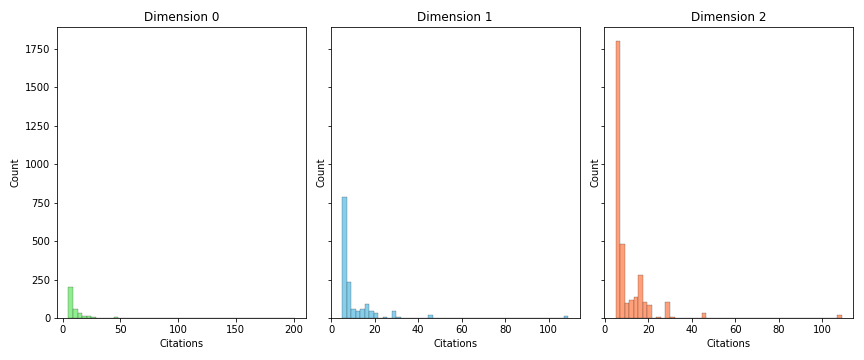
\includegraphics[scale=0.35]{./figures/distribution_cohain_150250.png}
% \caption{Distribution of the citation in CC1 } \label{fig:accuracy}
%\end{figure}
\begin{figure}[tb]
\centering
 \begin{subfigure}[t]{-0.8\textwidth}
 \vspace{-4cm}
    \text{(a)}
  \end{subfigure}
\begin{subfigure}[t]{0.8\textwidth}
\centering
   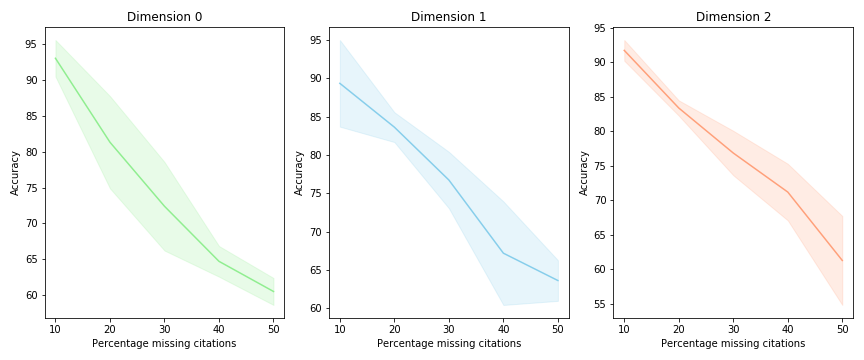
\includegraphics[scale=0.35]{./figures/accuracy_network1.png}
 %\caption{Accuracy of SNN in predicting missing citations } \label{fig:accuracy}
\end{subfigure}
 \begin{subfigure}[t]{0.8\textwidth}
    \text{(b)}
  \end{subfigure}
\begin{subfigure}[t]{0.8\textwidth}
\centering
\vspace{-0.5cm}
   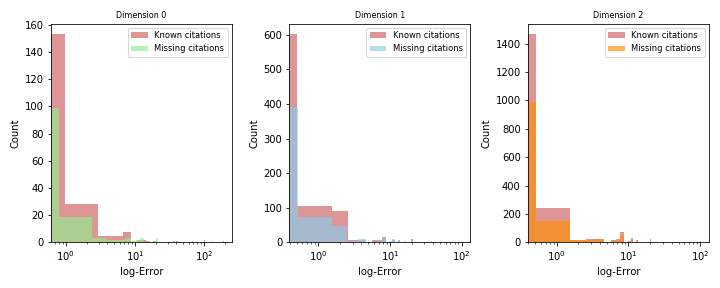
\includegraphics[scale=0.36]{./figures/Error_dist_start150250_seed6666_notsee40.png}
 % \caption{Distribution of the prediction's error} \label{fig:error}
\end{subfigure}
\caption{(a) Mean Accuracy $\pm$ std over 5 samples of SNN in imputing missing citations on CC1. (b)Mean Absolute Error $\pm$ std over 5 samples of SNN for $40\%$ missing values in CC1. \stefania{Add error on bins}}
\label{fig:accuracy-error}
\end{figure}
As a second assessment for our network we evaluate how accurately an SNN pretrained on a co-authorship complex can impute missing citations on a different complex. This is build over the assumption that co-authorship complexes share a similar structure. In Figure ~\ref{fig:transfer-learning} we show the MA in predicting missing citations on CC1 using the above architecture of SNN trained on CC2 (Co-authorship Complex 2, see Table~\ref{table:Simplices-coauthor}).
We compared our results with imputation methods based on statistical techniques, namely replacing missing data with the median or mean of the known data and inferring the missing values from the $(k-1)$ and $(k+1)$ neighbors of the simplices ($k$-simplicial neighbor $k$-sn). As Table~\ref{table:comparison-SNN} shows, SNNs outperform statistical techniques. Comparison with other state of the art imputations algorithms is left for future work.
\begin{figure}[htbp]
  \centering
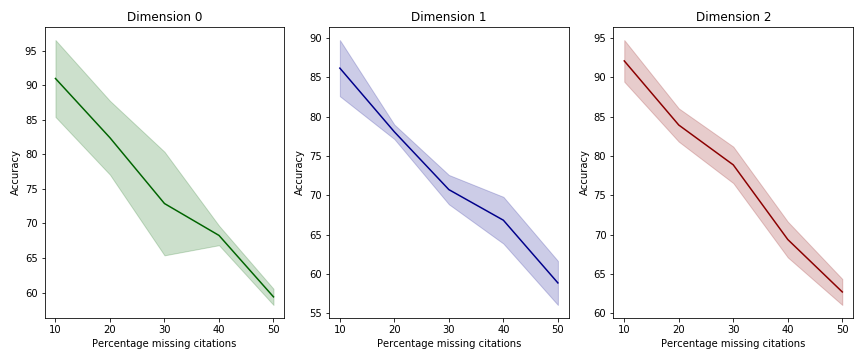
\includegraphics[scale=0.35]{./figures/accuracy_network1_pretrained.png}
  \caption{ Mean Accuracy $\pm$ std over 5 samples in imputing missing citations on CC1 of SNN trained on CC2 . } \label{fig:transfer-learning}
\end{figure}

%\scriptsize{
\begin{table}[htbp]
  \label{table:comparison-SNN}
  \centering
  \scriptsize{
  \begin{tabular}{c|cccccc}
    \cmidrule(r){1-7}
    Method   & CC1 - dim 0   & CC1 - dim 1   & CC1 - dim 2   & CC2 - dim 0  & CC2 - dim 1  & CC2 - dim 2 \\
    \midrule
    Mean & 1  & 12 & 1  & 1 & 1  & 1\\
    Median & 16 & 50 & 1  & 1& 1  & 1\\
    $k$-sn & 16 & 50& 1  & 1& 1  & 1 \\
    \bottomrule
  \end{tabular}}
  \caption
